\documentclass{article}
\usepackage[utf8]{inputenc}
\usepackage{graphicx}
\title{
\includegraphics[width=0.5\textwidth]{UU_logo.pdf}\\
Construction of the Slidarr}

\author{Mats Jonsson, Sören Meinken, Mohammad El Musleh}
\date{March 2019}

\begin{document}

\maketitle

\section{Introduction}
The idea is to create a new revolutionary musical instrument called Slidarr. It originated from using the guitar instrument but instread of pulling the strings, the fingers will slide on the strings without the strings making any sound. The sound will come from the relative location of the fingers on the strings which will be determined by the electronic equipment developed in this project.

Since the construction of the actual instrument is very simple, just some strings and and wires, it can be build in many different ways. For example, it can be attached to a steel-stringed guitar, but also built as a one-stringed guitar or like a violin with a conductive bow.

\section{Objectives}
On a guitar there are usually six strings, but this instrument only needs one or two strings to operate. In addition to that, the project will be started using optimal conditions for the strings and the conductor on the hand. This means using a very good conductor on the finger to bridge the strings, so that the biggest resistance is the length of the wires. If this works, the next move would be to use bare hands with possibly other strings that have a similar resistance. Once the MIDI data is created from the ADC there are several options what to do with it e.g. send it to a computer/syntheziser via USB, wirelessly or synthezise the signal on chip.

\begin{figure}[h]
  \centering
  %  \vspace*{-0.15in}
  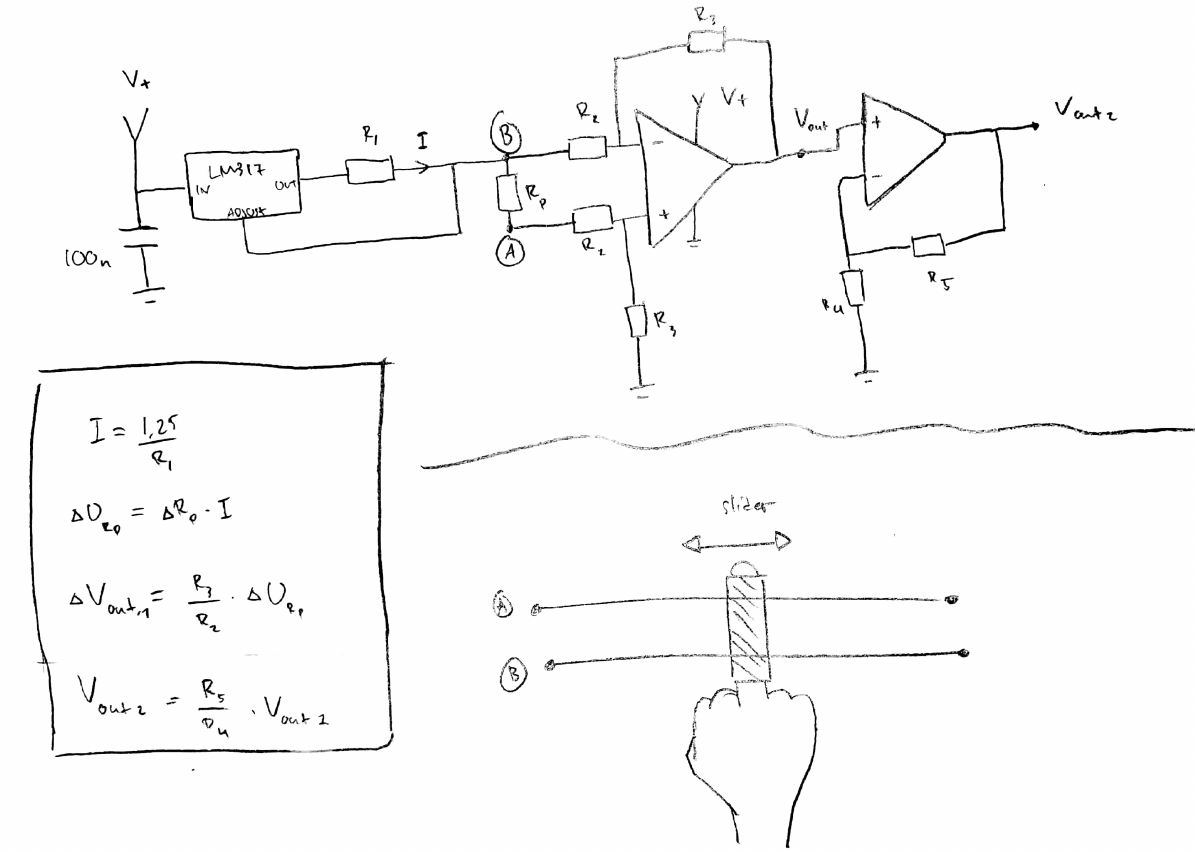
\includegraphics[width=0.9\textwidth]{circuit.png}
  \caption{Circuit diagram and principal sketch for the Slidarr.}
  \label{fig:circuit}
\end{figure}

\section{System overview}
The Slidarr senses tiny changes in resistance and translates it to MIDI commands, before sending them over USB to a computer running an software synth that produces the audio. The instrument's interface will consist of a metal wire with a constant current running through it. See figure \ref{fig:circuit}. The artist touches the wire at any position with a conductor, further called the "finger", that reads a tiny voltage drop depending on its position along the wire. The voltage drop between A and B is amplified using the presented circuit, and fed into an ADC converter on the ARM Cortex that translates the signal to the corresponding MIDI note. 

\subsection{User interaction}

When the finger makes contact with the string, the system sends a "note on" event. The finger can now slide along the wire, resulting in continuous "pitchbend" events that are able to change the frequency of the tone generated by the synth. When the finger is released, an "note off" event is sent.

A button implements a scrolling feature. When the button is pressed, sliding the finger along the string will "scroll" the frequency range covered by the string up or down the scale, allowing the artist to reach higher or lower notes with just a short string.

\subsection{Calibration}
The artist should be able to calibrate the system. Another button lets the artist define two positions of the string that correspond to one octave.

\section{Organisation}

There are five major parts in this project to be realized:
\begin{itemize}
    \item Creating/developing a measurement circuit to read the resistance(distance) from the strings
    \item Read that signal with an ADC
    \item Convert the signal to a proper representation for the MIDI protocol
    \item Send the signal to a syntheziser
    \item Calibration and setting of modes
\end{itemize}

Hardware needed:
\begin{itemize}
    \item strings
    \item circuit
    \item microcontroller with ADC
    \item calibration buttons, leds for mode?
    \item USB or wifi tranceiver (or only transmitter?)
\end{itemize}

The five major parts mentioned before can all be developed on in parallel. There will be three people working available to work in this project.

\section{Method}

\section{Challenge}
To get a proper measurement so that notes can be created from it and beautiful music is created.

\end{document}
